%!TEX TS-program = xelatex  
%!TEX encoding = UTF-8 Unicode  
\documentclass[a4paper, 11pt]{article}
\usepackage{ctex}
\usepackage[margin=1in]{geometry}
\setmainfont{HiraginoSansGB-W3}
\setCJKmainfont{HiraginoSansGB-W3}
\setCJKsansfont{HiraginoSansGB-W3}

\usepackage{graphicx}
\usepackage{subfigure}
\usepackage{listings}
\lstset{language=C++} 

\begin{document}

\title{Badkid: ELF文件病毒设计报告}

\author{柯嵩宇,陈天垚,万诚,杨闰哲\vspace{1em} \\ 2014级ACM班}
\maketitle

这篇文档的目的,在于还原我们小组对我们的ELF文件病毒“badkid”的设计过程,以及我们在整个设计过程中的技术思考。但请原谅,我们不会在此文中专门介绍ELF文件格式等网上随处可搜到的内容,而是力图忠实地记录我们在实现设计目标中“走过的弯路”与“乍现的灵光”,希望以此给那些想要亲自动手写一个ELF文件病毒(或是想要对抗此类病毒)读者,带来一些有益的启发。

\tableofcontents
\newpage
\section{项目简介}
	~~~~~~此项目中,我们的目的是设计一个感染ELF文件的寄生病毒:当一个ELF文件受其感染时,会修改它的头入口点(entry point);当用户运行一个被感染文件时,就会先执行病毒代码,感染同目录下的其他文件,从而达到复制与传播的效果。寄主程序运行顺序的执行顺序如图\ref{fig:order}所示。
	\vspace{1em}
	\begin{figure*}[htbp]
		\centering
		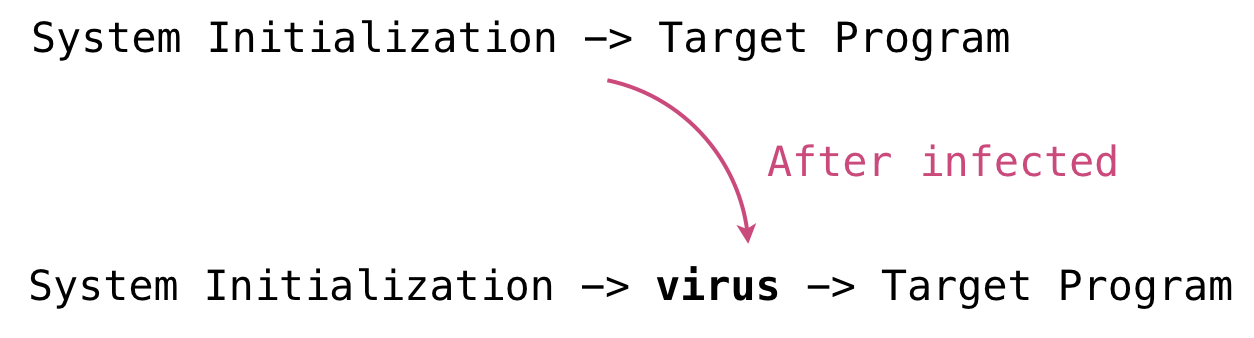
\includegraphics[width = \textwidth]{figures/fig3_first}
		\caption{受感染寄主程序的执行顺序}
		\label{fig:order}
	\end{figure*}
\subsection{环境假设}	
	~~~~~~我们假定病毒工作于以下环境:
	\begin{enumerate}
		\item 指令集架构:x86\_64
		\item 操作系统:Linux
		\item 被感染文件在root权限下运行
	\end{enumerate}
	
	同时我们假定了一个可获得的root权限,因为这样可以让我们专注于ELF文件的分析与重构、病毒的攻击行为与连接病毒本身,而不用操心其他问题。另外,我们选择用C语言写病毒代码,而不是C++,因为C++在编译的时候会包含全局的初始化,这会给改写ELF的过程增添不少麻烦。

\newpage
\section{主要技术}
~~~~~~设计一个ELF病毒的核心问题是,如何寄生我们的ELF病毒。如果我们直接让病毒直接覆盖宿主,受感染后的宿主文件被破坏,即让它覆盖可执行文件,破坏原始数据。这种传染方式将导致下次宿主程序执行失败,病毒很易被发现。如果被破坏的宿主是系统赖以生存的重要文件,将导致整个系统崩溃。我们更希望在向宿主文件中插入病毒体时,不破坏宿主主体,修改程序流程,以便病毒跟随宿主一起执行。这种情况下寄生病毒不改变宿主内部对象格式,在自身得到执行后将控制交还给宿主。但是如何把病毒体嵌入宿主文件中呢?是静态链接还是动态链接?我们嵌入后的病毒执行后如何执行原来的文件呢?我们做了一下尝试。
\subsection{初尝试:一个静态病毒?}
~~~~~~我们最开始的想法是用静态链接嵌入我们的病毒。如果把程序希望把自己的代码编译成静态的,这样在嵌入文件的时候就不需要考虑载入外部文件时的问题,只需要修改一些位置就可以执行代码了。如:ELF的EntryPoint,\_start()函数等。但是这样有可能造成的是,如果自己与目标程序的内存使用存在重叠,那么就无法正常嵌入代码。
\vspace{1em}
	\begin{figure*}[htbp]
		\centering
		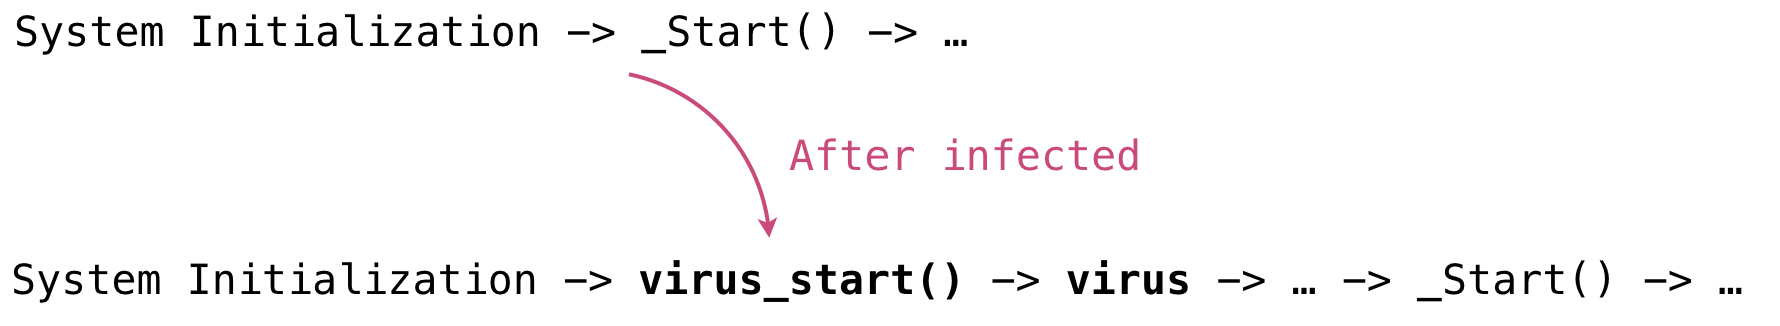
\includegraphics[width = \textwidth]{figures/fig1_order}
		\caption{静态链接病毒}
		\label{fig:way1}
	\end{figure*}
\subsection{PIE:位置无关可执行文件}
~~~~~~经历过上面的尝试后我们想到,应该用Poistion Indipendent Executable (PIE),病毒体使用位置无关代码,如果宿主地址空间从0x08048000到0x08049000,病毒体就使用0x08048000之前或者0x08049000之后的地址。病毒体必须是位置无关的,因为它无法知道最后所用地址,直到成功感染了宿主之后。这种技术的主要好处在于病毒体可以驻留内存,而第一种方式病毒体只能执行一次,然后就将控制权交还给宿主了,自身为原宿主所替换。

但是在GCC的编译选项中,PIE和static是冲突的,即PIE代码一定是动态链接的,这样一来就造成了一些麻烦。我们尝试了用一个程序把一个PIE-ELF文件的内存布局向后偏移0x200000的位置。但如果只是修改Segments中的信息是不够的,首次的尝试失败了。后面我们查到了使用动态链接的程序在执行的时候回读取DYNAMIC段的信息,里面包含了一些绝对地址的项,然后通过在代码中添加修改相应项的信息的代码,使得偏移之后的代码可以正常执行了!

\subsection{使用一个Wrapper}
~~~~~~通过动态链接使我们的代码正常执行后,我们尝试把两个ELF(病毒与宿主文件)连在一起。但这个时候就出现了又一个困难。我们原本以为只需要把Segments的信息合并即可,但是事实却不尽人意。当我们把两个ELF连接到一起之后,发现程序其实无法正常执行,使用readelf读取合并后的ELF文件,获得警告信息(程序中有两个DYNAMIC段)。这就意味着,如果我们的病毒是一个PIE的话,它就只能注入到静态连接的代码中,这就大大地缩小了我们病毒的感染范围。
	\begin{figure*}[htbp]
		\centering
		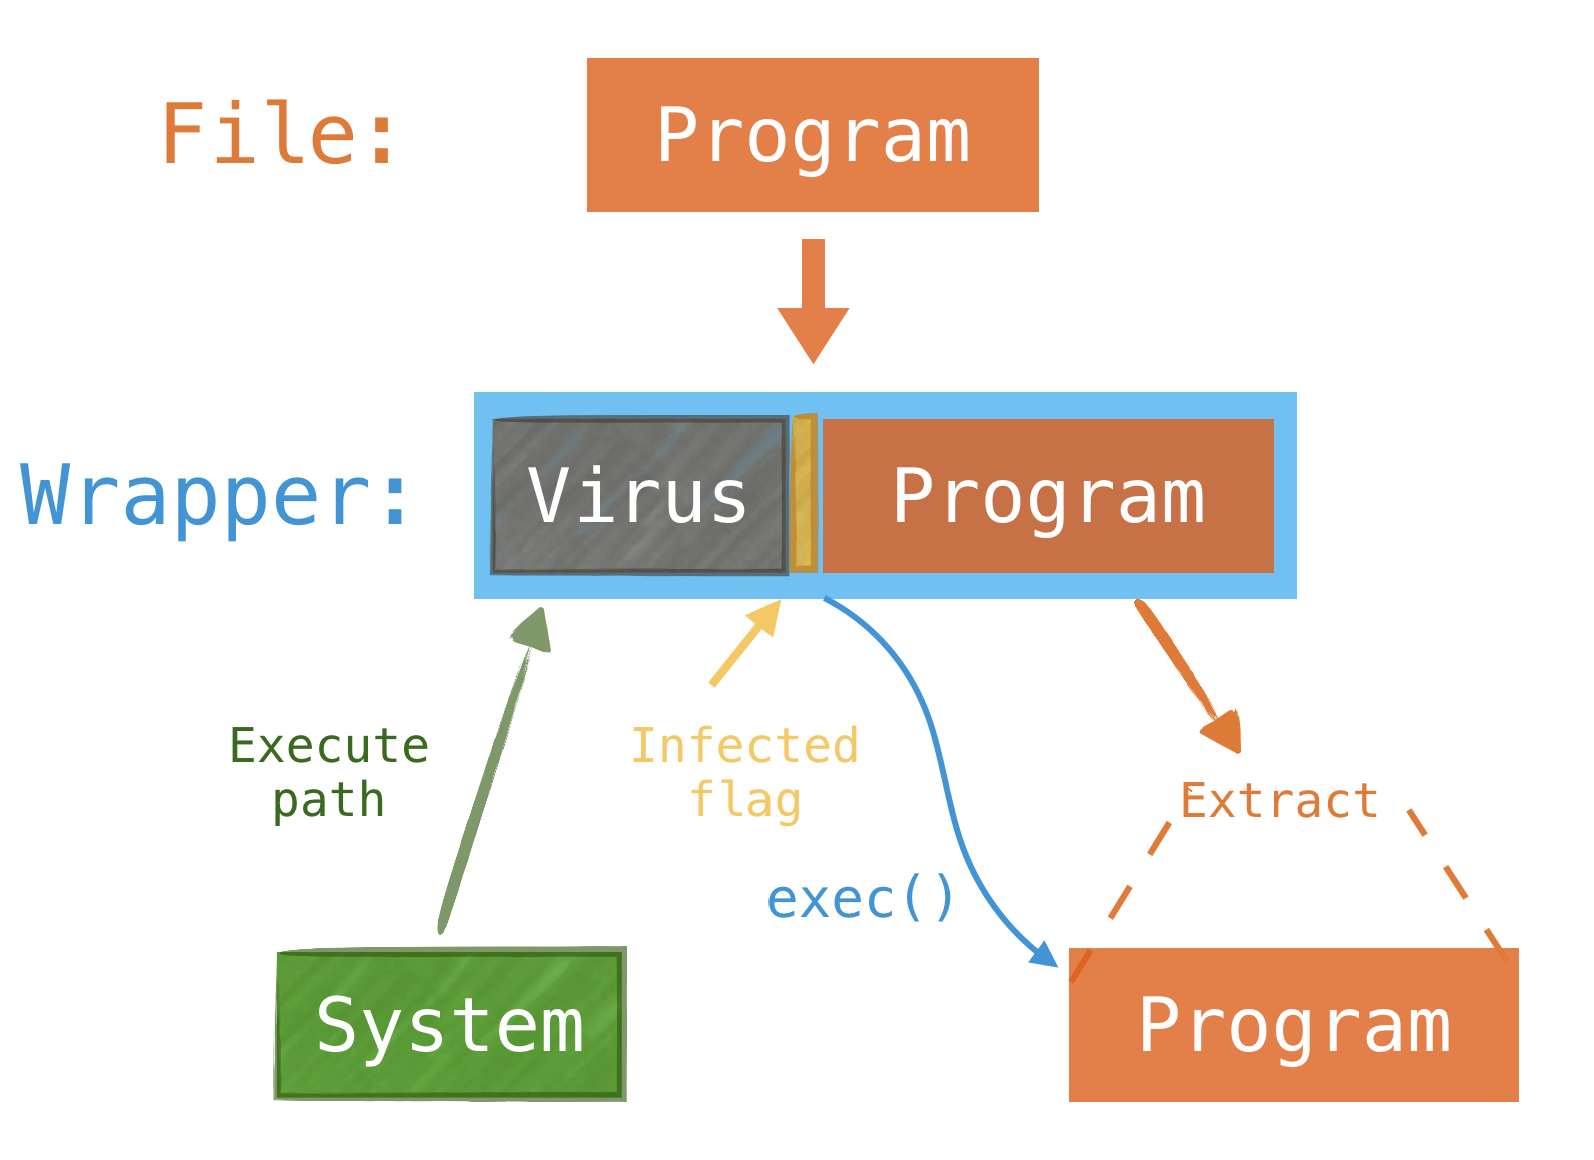
\includegraphics[width = \textwidth]{figures/fig2_wrapper}
		\caption{用一个Wrapper把宿主文件放在病毒后}
		\label{fig:way3}
	\end{figure*}
然后我我们就只好放弃之前的做法,做了一个非常简单却巧妙的尝试。我们使用一个Wrapper,把原来的ELF(宿主文件)添加在新的ELF(病毒)的16KB之后的位置,16KB之前的为病毒的ELF文件信息,这样一来,病毒在执行的时候会读取自己16KB之后的文件,然后输出到/tmp目录下面一个文件名随机的文件中,然后再用fork,exec这两个系统调用执行宿主程序。

\subsection{终极思路:感染共享库}
~~~~~~经历了上面的种种尝试之后,我们想到,能不能把修改程序的DYNAMIC段信息,添加一个共享库的依赖,然后把我们的病毒代码放在某个共享库的初始化代码中,这样操作系统在加载被感染的代码的时候就会加载所有被依赖的共享库并且执行共享库的初始化操作。这样只需要对目标ELF作出少量修改即可完成我们的目标。

\begin{figure*}[htbp]
		\centering
		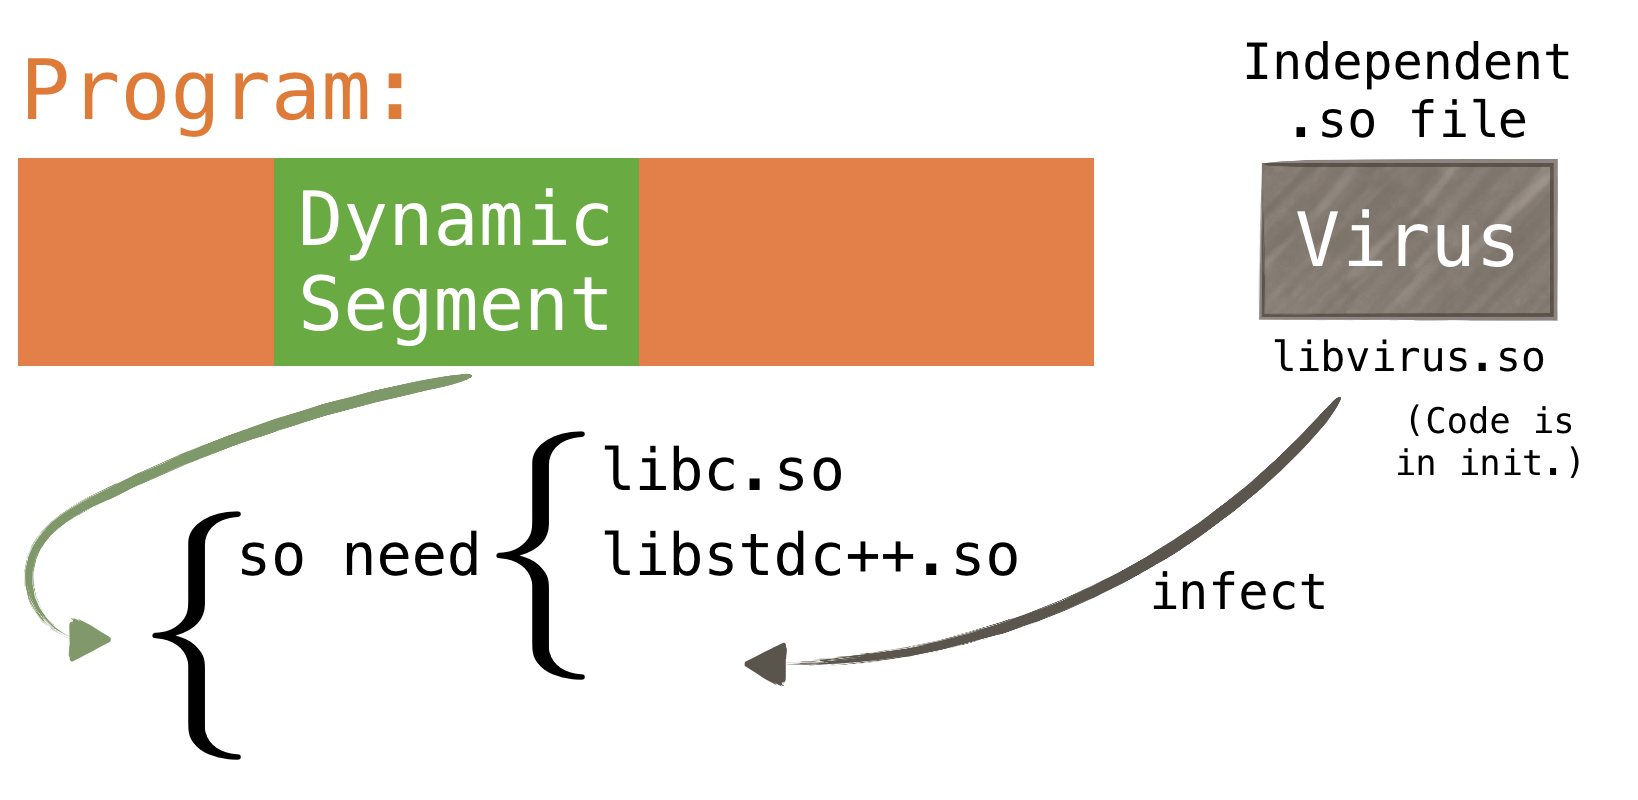
\includegraphics[width = \textwidth]{figures/fig4_ld1}
		\caption{感染共享库思路示意图}
		\label{fig:way4}
\end{figure*}

由于ELF文件在只读内存(程序,字符串等)的排列是非常紧密的,通过自己编写ELF读写代码的工作量就变得非常大。我们在Google搜索能够读写ELF文件的库时,找到了我们现在所使用了ELFIO这个库,这个库是由C++编写成的(虽然在一开始由于C++程序初始化比较复杂的原因,我们决定的是只写C代码,但是由于我们改变了我们感染文件的策略,写C++代码也就变得不是那么不可以接受了...)。 而且一个意外的好处是:这个库并不需要特殊共享库的支持,所有用到的共享库都是Linux系统必然自带的。这给我们的项目带来了巨大的便利。

我们编写相关的代码,把代码编译成共享库(g++ source.cc -o libsource -shared -fPIC -...),然后通过dlopen函数手动加载共享库并成功的执行了写在初始化部分的(C++全局对象的构造函数)病毒代码。这一成功给了我们极大的信心。然后我们开始编写搜索ELF文件中.dynstr和.dynamic信息的代码,然后试图修改并写回文件(在实验中,为了区别感染与未感染,我们感染后的输出并不是原文件)。我们尝试获得了成功。
\begin{figure*}[htbp]
		\centering
		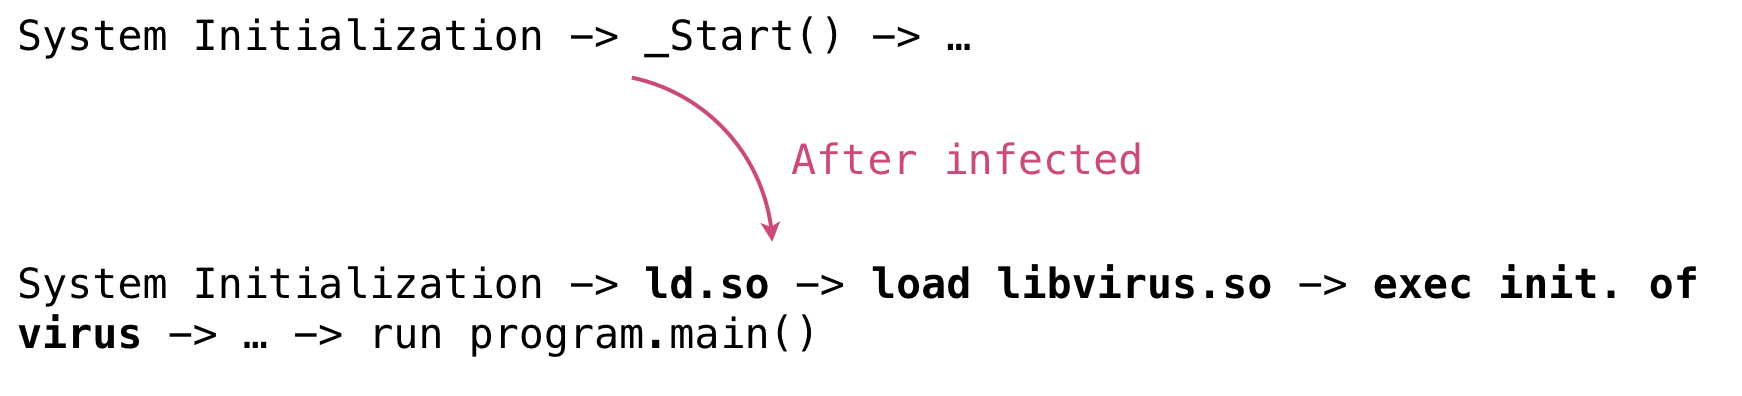
\includegraphics[width = \textwidth]{figures/fig5_ld2}
		\caption{感染前后执行路径对比}
		\label{fig:way4}
\end{figure*}

\section{具体实现}
关于包装这个病毒,首先是手动的版本,手动把文件复制到/lib/x86\_64-linux-gnu目录下,然后使用一个调用dlopen函数加载指定so文件的程序激活病毒。我们也写了一个能够把so文件的内容按字节用转义字符变成C的字符串,以数据的形式放在一个程序中,这个程序在运行的时候会在/lib/x86\_64-linux-gnu目录下创建libvirus.so文件,并且写入正确的信息。然后通过dlopen加载SO执行病毒代码。

我们尝试了多线程、多线程地感染的支持。我们先把原来单线程的感染操作(在初始化的时候扫描目录,感染文件)改成了多线程。但是因为特殊的原因,单进程多线程的做法并不能满足我们的要求。最后我们使用了多进程的方法来实现不阻塞的感染。幸运的是,由于我们是一个so文件,调用fork之后通过ps查看到的只是原程序的路径,这样可以欺骗用户是他们用特殊方法执行了两次程序。

\subsection{源码解析}

\subsection{一些实验}
\section{小结}

\end{document}
